\chapter[Revisão de Literatura]{Revisão de Literatura}

%\addcontentsline{toc}{chapter}{Revisão de Literatura}
% ----------------------------------------------------------

Nesse capítulo é feita uma revisão no estado da arte de diferentes formas de utilizar os algoritmos de busca, algoritmos genéticos, paralelismo ou uma união de todas ao mesmo tempo.

\section{Busca Heurística}

Busca heurística de caminhos é um subgrupo de algoritmos de busca em grafos \cite{Winston}, é um mecanismo geral de solução de problemas no ramo de IA. A sequência de passos necessários para solução da maioria dos problemas de IA usualmente não é conhecida, mas deve ser determinada por uma exploração de alternativas através de mecanismos de tentativa e erro. Um problema de busca típico é o PCV, que consiste em encontrar o caminho mais curto que as visite cada cidade de um conjunto cidades e retorne para a cidade de partida. Os algoritmos BFS e o A* são otimo exemplos de busca heurística. \cite{KORF199341}

\subsection{\textit{Best-first search}}

É um algoritmo de busca heurística geral. Ele mantém uma lista aberta contendo os nós ainda não visitados de uma árvore que é gerada, e uma lista fechada dos nós que já foram expandidos e visitados. Cada nó tem um valor de custo, em cada ciclo um nó de menor custo da lista aberta é expandido, cada filho do nó é avaliado por uma função de custo \ref{eq:FormulaHeuristicaBFS}  e adicionado na lista aberta, e o nó pai é adicionado a lista de nos fechados.

\begin{equation} \label{eq:FormulaHeuristicaBFS}
f(n) =  h(n)
\end{equation}

A lista aberta contem apenas o nó inicial e o algorítimo termina quando encontrar o nó de destino para expansão.\cite{KORF199341}

Existem muitas implementações com alterações do BFS, tais como \textit{Dijkstra} ou A*, o que os diferencia basicamente é como é implementada sua função de custo.

\subsection{O Algoritmo A*}

O algoritmo A* é um dos mais populares soluções no ramo de busca de caminhos, um desses motivos é que sempre garantindo achar o menor caminho entre dois pontos \cite{PEHart}, porém,  gera uma grande árvore de busca nos processos, consumindo muito tempo e memória. É comum haver modificações no algoritmo para explorar uma árvore de busca menor, diminuindo o tempo para achar um caminho sacrificando a garantia de se encontrar o melhor caminho no final. \cite{Botea}.
O algoritmo A*, em sua forma tradicional, utiliza a fórmula heurística \ref{eq:FormulaHeuristica}. 

\begin{equation} \label{eq:FormulaHeuristica}
     f(n) = g(n) + h(n)
\end{equation}

Onde g(n) é o custo para chegar ao nó n, e h(n) é o custo estimado para atingir o nó de destino a partir do nó n. Este sempre deve ser menor ou igual a distância real entre o ponto n e o destino, ou seja nunca pode ser super-estimado. Para cada iteração sobre os vizinhos do nó atual é calculado o f(n) e adicionado em uma lista de nós abertos (A), mantendo uma referência do nó que serviu de origem para chegar nele, caso o nó ja esteja na lista e o valor de f(n) novo for menor, o valor de f(n) e o nó de origem é substituído pelo novo. Depois é verificado na lista o menor valor de f(n), este é removido, adicionado a lista de nos fechados (F) e a partir desse ponto, ele se torna o nó atual, quando o nó atual é o mesmo nó de destino o algorítimo retorna o caminho encontrado, assim podemos encontrar a solução ideal. \cite{PEHart} 

Podemos aplicar o algoritmo A* em um Grafo direcionado ponderado por exemplo da Figura \ref{fig:GrafoBusca}.

\begin{minipage}{\linewidth}
    \makebox[\linewidth][c]{
        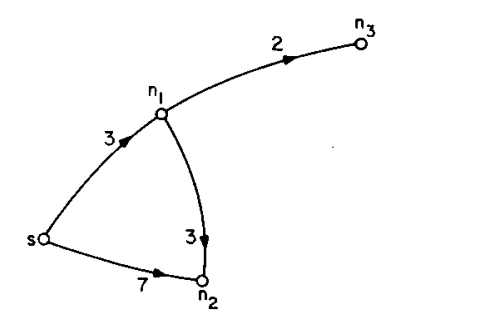
\includegraphics[keepaspectratio=true,scale=0.5]{ibagens/figura1.png}}
    \captionof{figure}{Grafo para busca \cite{PEHart}}
    \label{fig:GrafoBusca}
\end{minipage}

O grafo consiste em um nó inicial s e mais três outros nós (n1, n2, n3). As arestas contem a direção e o custo do trajeto. Se partirmos do algoritmo A* para produzir um subgrafo do melhor caminho, partindo de s podemos ir para n1 e n2, os valores de g(n1) e g(n2) são respectivamente 3 e 7. Supondo que A* expanda n1, sucedido por n2 e n3, nesse ponto g(n3)=3+2=5,o valor de g(n2) é diminuído pois um caminho de menor custo foi encontrado  3+3=6, o valor de g(n1) continua sendo 3.

O próximo passo seria estimar o h(n), podem essa função vai depender muito do domínio do problema, muitos problemas de encontrar o menor caminho entre dois pontos de um grafo possuem alguma "informação física" que pode ser usada de alguma forma para estimar o h(n), podemos em nosso exemplo, se definirmos como cidades ligadas por estradas, h(n) poderia ser a distancia aérea da cidade n até a cidade objetivo, essa distancia seria menor do que qualquer estrada da cidade n até o objetivo \cite{PEHart}. Em jogos digitais e buscas em tempo real é muito comum trabalhar em cima de mapas em forma de matrizes bidimensionais, esse será o foco dos algoritmos que trataremos, nesses casos fica simples tratarmos o h(n) com a distância Euclideana ou Manhattan entre n e o destino. \cite{Yngvi}

Quando definimos o mapa de busca em uma matriz bidimensional NxM, situação comum em jogos digitais e problemas de busca em tempo real \cite{Ross_Graham} \cite{Ulysses} \cite{Ulysses2}, precisamos definir os custos de movimentação entre os vizinhos do ponto n, e a função heurística h(n). O custo de movimentação na grade pode variar basicamente em dois tipos, levando as diagonais em consideração ou não.

O modelo em \textit{tile}, onde o movimento do agente está restrito a quatro direções ortogonais com custo 1, e \textit{octile}, onde o agente pode ainda mover-se na diagonal com custo equivalente ao valor da hipotenusa de um triângulo retângulo com catetos igual a 1, sendo assim  $ \sqrt{2}  \approx 1.4 $. É comum para fim de simplificar os cálculos multiplicar os valores de custo por 10 ou 100 como pode ser visto na Figura \ref{fig:CustoMovimento}.

\begin{minipage}{\linewidth}
    \makebox[\linewidth][c]{
        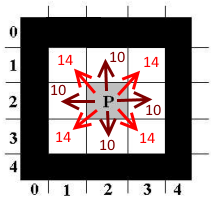
\includegraphics[keepaspectratio=true,scale=1.5]{ibagens/mov_cost.png}}
    \captionof{figure}{Custo de movimentação}
    \label{fig:CustoMovimento}
\end{minipage}

Uma heurística famosa e muito utilizada é conhecida como distância Manhattan, usada principalmente em ambientes de grades, ela estima a distância real entre os nós pela soma do deslocamento vertical e horizontal entre dois pontos, ignorando qualquer obstáculo.
A distância Manhattan garante a solução com mais baixo custo, pois cada nó deve caminhar pelo menos, a sua distância Manhattan, e o movimento é dado de um nó por vez \cite{Korf2000}.

Ainda pode ser facilmente modificado para levar em conta o produto vetorial entre o vetor do ponto inicial e o vetor de objetivo, resultando em um caminho reto entre dois nós. \cite{GameProgrammingHeuristics}.

Ainda pode ser realizada uma alteração no algoritmo de distância Manhattan para levar em conta as diagonais, este fica chamado de distância diagonal, adicionando um custo de movimentação diagonal diferente ao de movimentação adjacente.

Também pode ser utilizada como função heurística a distância euclideana, no entanto, neste caso teremos problemas com o uso de A*, pois a função de custo g não irá corresponder a função heurística h, ja que a  distância euclidiana é mais curta do que Manhattan ou a distância diagonal, você ainda terá os caminhos mais curtos, mas o A* levará mais tempo para ser executado \cite{GameProgrammingHeuristics}.

Podemos verificar na Figura \ref{fig:Manhattan}, exemplos de distância Manhattan comparado com a distância euclideana.

\begin{minipage}{\linewidth}
    \makebox[\linewidth][c]{
        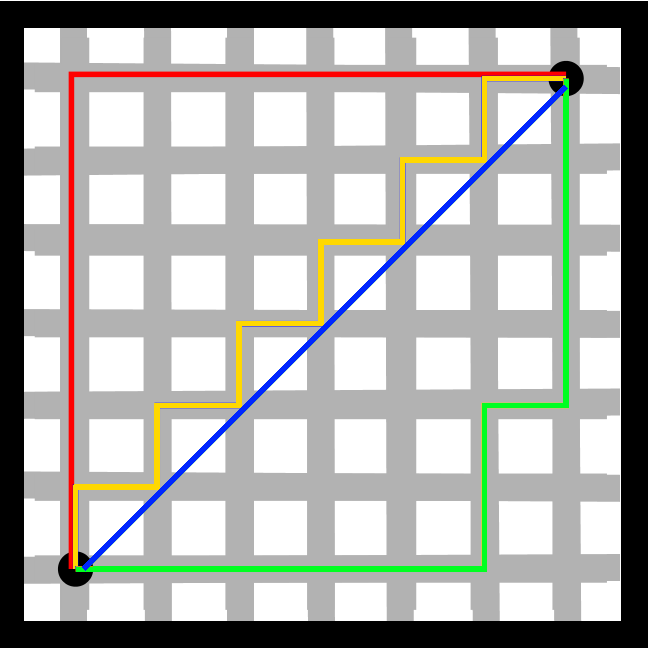
\includegraphics[keepaspectratio=true,scale=0.5]{ibagens/manhatam.png}}
    \captionof{figure}{Ilustração de diferença entre distância Manhatam e euclideana}
    \label{fig:Manhattan}
\end{minipage}

\begin{description}
    \item[Figura 4] As linhas de cor vermelho, verde e amarelo tem o mesmo tamanho (12), e representam a distancia Manhattan, a amarela leva em consideração o produto vetorial.
    A linha azul representa a distancia euclideana $\sqrt{72} \approx 8.485$
\end{description}

Uma limitação do A* é o fato requerer uma grande quantidade de recursos da CPU. Caso haja muitos nós a pesquisar, como é o caso em grandes mapas que são populares em jogos recentes, isso  pode causar pequenos atrasos.
Esse atraso pode ser agravado caso haja múltiplos agentes de inteligência artificial ou quando o agente tem que se mover de um lado do mapa para o outro 

Este alto custo de recursos da CPU pode fazer com que o jogo congele até que o caminho ideal seja encontrado. Game designers tentam superar esses problemas realizando ajustes nos jogos, de forma a tentar evitar estas situações \cite{Timothy}.

Pelo motivo do alto custo, a heurística fornece uma expansão considerável dos nós, que são mantidos na memória durante todo o processamento. A Figura \ref{fig:ExemploAStar} mostra a expansão da heurística.

\begin{minipage}{\linewidth}
    \makebox[\linewidth][c]{
        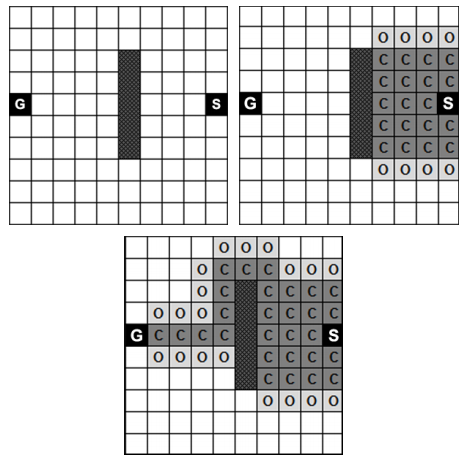
\includegraphics[keepaspectratio=true,scale=1]{ibagens/figura2.png}}
    \captionof{figure}{Exemplo de A* \cite{Ulysses} }
    \label{fig:ExemploAStar}
\end{minipage}

É comum no meio dos jogos digitais termos mais de um agente rodando ao mesmo tempo, um otimização para esse problema, proposta por Ko- Hsin, Cindy Wang e Adi Botea, examina o planejamento de caminhos multi-agente. Eles propõem um algoritmo chamado de FAR (\textit{Flow Annotation Replanning}) para combater os problemas técnicos envolvidos em pesquisas globais por várias entidades.
FAR implementa restrições de fluxo para evitar colisões frontais, para assim reduzir o espaço de busca que uma entidade deve considerar quando planejar a sua rota. Esse método tem a possibilidade de entrar em \textit{deadlock}, um estado de bloqueio, porem o algoritmo é capaz de contornar esse problema \cite{Ko-hsin}.

É comum a utilização do BFS apenas, como possui uma função heurisitica mais simples consome menos memoria, porem não garante a certeza do melhor caminho. \cite{UlyssesTCC}\cite{Russell}.

Outra solução é o uso de metaheurísticas para a adaptação do algoritimo de busca ao ambiente. São estratégias de alto nível que guiam os processos de pesquisa, e tem como objetivo explorar, de forma eficiente, o espaço de busca, a fim de encontrar soluções ideais tanto para problemas simples, quanto  complexos. São técnicas não determinísticas e
podem utilizar heurísticas para guiar seu processo de pesquisa. São exemplos de metaheurísticas, Algoritmos Genéticos (AG), BuscaTabu, Colônia de Formigas, GRASP, Simulated Annealing, dentre outras. \cite{Blum}

Korf propôs o algoritmo Iterative Deepening A* (IDA*) \cite{Korf85}, o mesmo utiliza a busca em  profundidade combinada com a heurística do A*. O resultado é um algoritmo que encontra a solução ótima, com o gasto mínimo de memória. Essa tecnica tem como desvantagem gerar uma árvore na busca a cada iteração. Com isso, o algoritmo exige muito processamento, o que pode tornálo mais lento que o A* em determinados casos.

Em contraponto temos a proposta apresentada por Björnsson \cite{Bjornsson}, o Fringe Search, visa otimizar o algoritmo IDA*. O foco é eliminar a principal deficiência do IDA* já citada. De forma que a cada iteração, não é mais necessário gerar a árvore  novamente, pois o algoritmo armazena os nós folhas da mesma, o que faz que, na próxima iteração, a busca se inicie a partir desses nós. Com isso, o algoritmo Fringe Search consegue ser mais rápido
que o IDA*.

O Recursive Best–First Search (RBFS), proposto por Korf \cite{Korf92}, é um algoritmo que trabalha com a redução do consumo de memória para o processo de busca de caminhos. Este algoritmo utiliza a mesma heurística do BFS e promove uma otimização espacial para o mesmo.

A técnica de reconhecimento de padrão de obstáculos do ambiente é um assunto tratado por Demyen e Buro \cite{Demyen}. O algoritmo por eles proposto, chamado de Triangulation Reduction A* (TRA*), utiliza uma abstração do ambiente a fim de determinar o padrão dos obstáculos do ambiente. Este visa otimizar o tempo gasto no processamento do algoritmo A*. Esse método tem como desvantagem, requisitar um formato específico dos obstáculos do ambiente, que devem ser poligonais, o que pode inviabilizar sua utilização em
qualquer tipo de ambiente.

A arte de busca de caminhos está longe de um trabalho perfeito e muito ainda precisa ser feito \cite{Pontevia}.

\subsection{Aplicações}
Aplicações para os algoritmos de busca podem ser diversos, como por exemplo, em um simulador de carro corrida \cite{JungTing}. Utilizando o algoritmo do A* com duas modificações para encontrar o melhor caminho enquanto evita os obstáculos entre o ponto de início e o ponto de destino. 
A primeira modificação consiste em utilizar o teorema de Pitágoras, onde primeira calcula a distância entre dois pontos(1 e 2), verifica se existe algum obstáculo dentre eles, se existir, utiliza o terceiro ponto para calcular a hipotenusa e verifica se existe obstáculo entre a hipotenusa, se não existir, remove o ponto 2 e começa a considerar o caminho do ponto 1 para o ponto 3. A segunda modificação consiste em somente ir para frente, isso significa, procura somente os pontos a frente do carro, direita, esquerda e frente, simulando um controle de carro.

O projeto utiliza 3 pistas reais de corrida da Formula 1, Peru, Itália e Hungria, sendo cada pista, uma imagem de escala 1280x782 \textit{pixels} retiradas do site oficial da Formula 1. O Carro é implementado em \textit{Microsoft XNA Game Studio}, plataforma usada para desenvolver jogos para \textit{Windows Phone, Xbox e Windows}. As Imagens das pistas são modificadas para serem mapas de detecção de colisão, a pista é pintada de preto, indicando onde o carro pode andar e o resto pintado de branco indicando os o carro não pode andar. O carro tem o tamanho de 18x12 \textit{pixels} e uma movimentação de 2 \textit{pixels} por segundo. Como o XNA trabalha com uma taxa de quadros de 60 quadros por segundo, o carro se movimenta a 120 \textit{pixels} por segundo.A Figura \ref{fig:GameCarPista} mostra um exemplo de rota gerada na pista do Peru.

\begin{minipage}{\linewidth}
	\makebox[\linewidth][c]{
		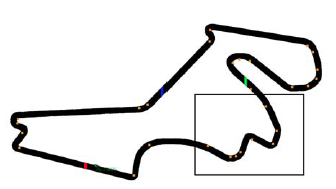
\includegraphics[keepaspectratio=true,scale=1.0]{ibagens/GameCarPista.png}}
	\captionof{figure}{Pisca de formula 1 do Peru \cite{JungTing} }
	\label{fig:GameCarPista}
\end{minipage}

Os resultados obtidos por \cite{JungTing} na primeira modificação conseguiu economizar ciclos de CPU, reduzindo o numero de pontos indicadores da pista em 97\%. A segunda modificação tem a vantagem de obter o tempo de volta mais curto, por que reduz o numero de nós do algoritmo A* de 4 para 3 nós]. A desvantagem é que o carro pode balançar em curvas acentuadas. Em geral, as modificações garantiram uma melhoria em performance, economizando o numero de ciclos de CPU.


\section{Algoritmo paralelo de busca}

O problema de busca de caminho pode ser facilmente quebrado em duas maneiras \cite{WilliamMiller}.

A primeira abordagem seria iniciar a busca  de ambos os nós, inicial e final simultaneamente, Esta variação do A*, também conhecida como Pesquisa Bidirecional, permite que um problema seja dividido em dois núcleos, mas não escala facilmente com um maior numero de núcleos ou com um problema de maior tamanho. Esta abordagem requer dois núcleos livres por busca, e não seria capaz de executar em um ambiente que não ofereça no mínimo essa estrutura. \cite{Janie_Chang}.

A segunda abordagem seria tratar cada busca de caminho como uma unidade individual e distribuir cada uma para um núcleo.
Esta abordagem funciona facilmente com qualquer número de núcleos e é possivelmente a forma mais eficaz de distribuição de grandes conjuntos de dados \cite{Jad} \cite{WilliamMiller}.


\section{Algoritmos genéticos}

AG é uma técnica amplamente utilizada de IA, que utilizam conceitos provenientes do princípio de seleção natural para abordar uma  ampla série de problemas, geralmente de adaptação. \cite{DiogoCLucas}

\subsection{Funcionamento}
 
Inspirado na maneira como o seleção natural explica o processo de evolução das espécies, Holland \cite{Holland1975} decompôs o funcionamento dos AG em sete etapas, essa são \textit{inicialização}, \textit{avaliação}, \textit{seleção}, \textit{cruzamento}, \textit{mutação}, \textit{atualização} e  \textit{finalização} conforme a Figura \ref{fig:EstruturaAG}. 

\begin{minipage}{\linewidth}
	\makebox[\linewidth]{
		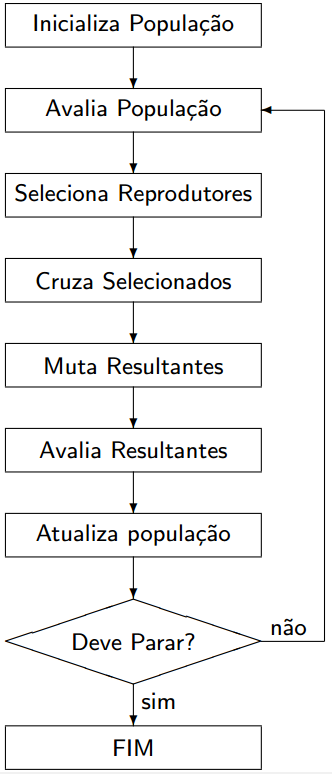
\includegraphics[keepaspectratio=true,scale=0.45]{ibagens/genetico1.png}}
	\captionof{figure}{Estrutura de um AG \cite{DiogoCLucas} }
	\label{fig:EstruturaAG}
\end{minipage}


Cada etapa do AG funciona da seguinte forma:

\textbf{Inicialização}: Criar uma população de possíveis respostas para um problema. 
É comum fazer uso de funções aleatórias para gerar os indivíduos, sendo este um recurso simples que visa fornecer maior diversidade.

\textbf{Avaliação}: Avalia-se a aptidão das soluções, os indivíduos da população, então é feita uma análise para que se estabeleça quão bem elas respondem ao problema proposto.
A função de avaliação também pode ser chamada de função objetivo. Ela pode variar de acordo com problema,  
Calcular com exatidão completa o grau de adaptação dos indivíduos pode ser uma tarefa complexa em muitos casos, e se levarmos em conta que esta operação é repetida varias vezes ao longo do processo de evolução, seu custo pode ser consideravelmente alto. Em tais situações é comum o uso de funções não determinísticas, que não avaliam a totalidade das características do indivíduo, operando apenas sobre uma amostragem destas.

\textbf{Seleção}: Ela é a responsável pela perpetuação de boas características na espécie. 
Neste estágio que os indivíduos são escolhidos para posterior cruzamento, fazendo uso do grau de adaptação de cada um é realizado um sorteio, onde os indivíduos com maior grau de adaptação tem maior probabilidade de se reproduzirem.
O grau adaptação é calculado a partir da função de avaliação para cada individuo, determina o quão apto ele esta para reprodução relativo a sua população. 

\textbf{Cruzamento}: Características das soluções escolhidas na seleção são recombinadas, gerando novos indivíduos.

\textbf{Mutação}: Características dos indivíduos resultantes do processo de reprodução são alteradas, acrescentando assim variedade a população.
A mutação opera sobre os indivíduos resultantes do processo de cruzamento e com uma probabilidade pré-determinada efetua algum tipo de alteração em sua  estrutura. A importância desta operação é o fato de que uma vez bem escolhido seu modo de atuar, é garantido que diversas alternativas serão exploradas.
 
\textbf{Atualização}: Os indivíduos criados no processo de reprodução e mutação são inseridos na população.

Na forma mais tradicional deste a população mantém um tamanho fixo e os indivíduos são criados em mesmo número que seus antecessores e os substituem por completo. 

Existem, porém, algumas alternativas, o número de indivíduos gerados pode ser menor ou o tamanho da população pode sofrer variações e o critério de inserção pode variar, por exemplo, nos casos em que os filhos substituem os pais, ou em que estes só são inseridos se possuírem maior aptidão que o cromossomo que sera substituído, ou o manter sempre o conjunto dos n melhores indivíduos. 

\textbf{Finalização}: É testado se as condições de encerramento da evolução foram atingidas, retornando para a etapa de avaliação em caso negativo e encerrando a execução em caso positivo.

Os critérios para a parada podem ser vários, desde o número de gerações criadas até o grau de convergência da população atual.


Toda base dos AG se fundamenta nos indivíduos, eles são a unidade básica em qual o algoritmo se baseia, sua função é codificar as possíveis soluções do problema a ser tratado e partir de sua manipulação no processo evolutivo, a partir daí que são encontradas as respostas.

Esses indivíduos precisam de uma representação, essa será o principal responsável pelo desempenho do programa. É comum chamar de \textit{genoma} ou \textit{cromossomo} para se referir ao individuo. Por essa definição podemos resumir um indivíduo pelos genes que possui, ou seja seu \textit{genótipo}.

Apesar de toda representação por parte do algoritmo ser baseada única e exclusivamente em seu genótipo, toda avaliação é baseada em seu fenótipo, o conjunto de características observáveis no objeto resultante do processo de decodificação dos genes do individuo, ver Tabela 1.

\newcolumntype{C}[1]{>{\centering\let\newline\\\arraybackslash\hspace{0pt}}m{#1}}
\begin{table}[h]
	\centering
\vspace{0.5cm}
\renewcommand{\arraystretch}{2.0}
\caption{Exemplos de genótipos e fenótipos correspondentes em alguns tipos de problemas \cite{DiogoCLucas}}
	\begin{tabular}{|C{4cm}|C{3.5cm}|C{7cm}|}
		\hline
		\textbf{Problema} & \textbf{Genótipo} & \textbf{ Fenótipo} \\
		\hline                  
		Otimização numérica & 0010101001110101 & 10869 \\
		\hline
		Caixeiro viajante & CGDEHABF & Comece pela cidade C, depois passe pelas cidades G, D, E, H, A, B e termine em F \\
		\hline
		Regras de aprendizado para agentes & C$_1$R$_4$C$_2$R$_6$C$_4$R$_1$ & Se condição 1 (C$_1$) execute regra 4 (R$_4$), se (C$_2$) execute (R$_6$), se (C$_4$) execute (R$_1$)\\
		\hline
	\end{tabular}
\end{table}	

Para cada indivíduo é calculado o seu grau de adaptação, a partir de uma função objetivo, comumente denotada como na formula \ref{eq:solve0}.

\begin{equation} \label{eq:solve0}
f_O(x)  
\end{equation}


Que vai representar o quão bem a resposta apresentada pelo individuo soluciona o problema proposto.

Também é calculado o grau de adaptação do indivíduo relativo aos outros membros da população a qual ele pertence, esse é chamado de grau de aptidão, para um indivíduo $x$ temos seu grau de aptidão denotado pela fórmula \ref{eq:solve1}.


\begin{equation} \label{eq:solve1}
	f_A(x) = \frac{f_O(x)}{ \sum_{i=1}^{n}  f_O(i)  }  
\end{equation}


 Sendo n o tamanho da população.
 
 A dinâmica populacional é a responsável pela evolução, ao propagar características desejáveis a gerações subsequentes no processo de cruzamento, enquanto novas são testadas no processo de mutação.
 
 Algumas definições importantes relativo as populações de um AG são:
 
 \textbf{Geração:} É o número de vezes em que a população passou pelo processo de seleção, reprodução, mutação e atualização.

\textbf{Média de adaptação:} É a taxa média que ao indivíduos se adaptaram ao problema, é definida pela formula \ref{eq:solve2}. 

\begin{equation} \label{eq:solve2}
M_A = \frac{ \sum_{i=1}^{n} f_O(i) }{n}
\end{equation}


\textbf{Grau de convergência:} define o qual próxima esta a media de adaptação desta população relativo as anteriores. O objetivo dos AG é fazer a população convergir para uma valor de adaptação ótimo.
Um estado negativo que pode ocorrer relativo a esta medida é a \textit{convergência prematura}, a mesma ocorre quando a população converge em uma média de adaptação sub-ótima, e dela não consegue sair por causa de sua baixa diversidade.

\textbf{Diversidade:} Mede o grau de variação entre os genótipos da população. Ela é fundamental para o tamanho da busca.
Sua queda esta fortemente ligada ao fenômeno de \textit{Convergência prematura}.

\textbf{Elite:} São os indivíduos mais bem adaptados da população. Uma técnica comum nos AG é p \textit{elitismo}, onde são selecionados k melhores indivíduos que serão mantidos a cada geração.

\subsection{Aplicações}
Existem vários aplicações para os algoritmo genéticos, por serem uma inteligência artificial não supervisionada, de rápido aprendizado e podendo ser paralelizado.

O modelo m-PRC(Problema de Rotas de Cobertura multi-veículo) é uma aplicação de algoritmos genéticos para construção de rotas em uma região mapeada, para encontrar uma boa distribuição de viaturas para patrulhamento urbano usado por departamentos de segurando como a policia, guardas municipais ou segurança privada \cite{Washington}. 
O Modelo é definido como um grafo não direcionado \ref{eq:solve3}. 

\begin{equation} \label{eq:solve3}
G=(V\cup W, E)
\end{equation}

Onde \ref{eq:solve4}: 

\begin{equation} \label{eq:solve4}
V\cup W
\end{equation}


Compõem o conjunto de vértices e E o conjunto de arestas, ou seja, o subgrafo induzido por E e um grafo completo cujo conjunto de nós é V. 
V são todos os vértices que podem ser visitados e é composto pelo subconjunto T, que são os vértices que devem ser visitados por algum veiculo. W é um conjunto de vértices onde todos os M veículos devem passar. M é o numero de rotas de veículos que começam no vértice base V$_0$. 

O m-PRC atribui o conjunto de m rotas de veículos com as restrições: todas as m rotas de veículos começam e terminam na base V$_0$, Tem exatamente m rotas, cada vértice de V pertence a no máximo uma rota, cada vértice de T pertence a exatamente uma rota, com exceção a base, cada vértice de W deve ter uma rota que passa por ele e em uma distancia C de um vértice V visitado, O modulo da diferença entre o número de vértices de diferentes rotas não pode exceder um determinado valor R. A Figura \ref{fig:GrafoVUW} mostra o grafo da relação de V com W.

\begin{minipage}{\linewidth}
	\makebox[\linewidth]{
		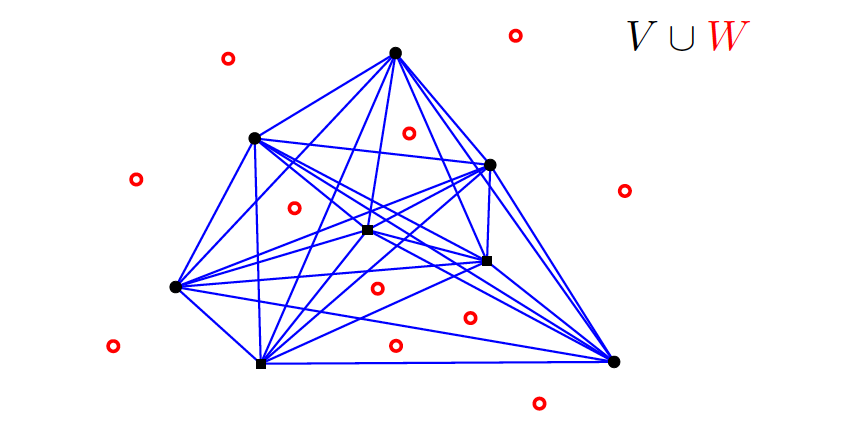
\includegraphics[keepaspectratio=true,scale=0.5]{ibagens/grafoMPRC.png}}
	\captionof{figure}{Exemplo de gráfo não direcionado para V U W. \cite{Washington} }
	\label{fig:GrafoVUW}
\end{minipage}

Para utilizar o algoritmos genéticos com o modelo m-PRC, o trabalho propõem dois modelos. O AGS (Algoritmo genético sequencial), que utiliza heurísticas GENIUS e 2-opt balanceada para ajustes finais para tentar melhor a solução; O AGH(Algoritmos genéticos H-1-PRC), que utiliza heurísticas H-1-PRC-MOD e 2-opt balanceada em todo o processo de resolução.

A conclusão de \cite{Washington} é que a utilização de algoritmos genéticos para a resolução de de uma adaptação do problema de rotas de cobertura de veículos como bastante relevantes e de fácil manipulação. O modelo AGS resolve o problema de forma rápida e tem uma fácil implementação dentro dos critérios de comparação adotadas. O modelo AGH é mais lento e não conseguiu encontrar a solução para alguns exemplos.

\section{Algoritmos genéticos para busca de caminhos}

Buscando melhorar a eficiência dos algoritmos de busca, foram criadas formas híbridas, onde utilizam inteligência artificial para analisar todo o percusso e ajudar o algoritmo de busca a decidir em momentos que a próxima ação é incerta.

Utilizando o algoritmo de busca BFS (\textit{Best First Search}), foi desenvolvido o modelo PPGA (\textit{Patterned based Pathfinding with Genetic Algorithm}). O modelo utiliza algoritmos genéticos como um módulo para calcular os sub-caminhos ao longo do processo de busca, cada vez que o módulo é chamado, herda informações da chamada anterior, tendo um ganha considerado de desempenho. O módulo é chamado, quando nenhum dos valores dados pelo BFS são melhores que o valor atual. A Figura \ref{fig:Fluxograma}  mostra uma fluxograma do funcionamento do modelo.

\begin{minipage}{\linewidth}
	\centering
	\makebox[\linewidth]{
		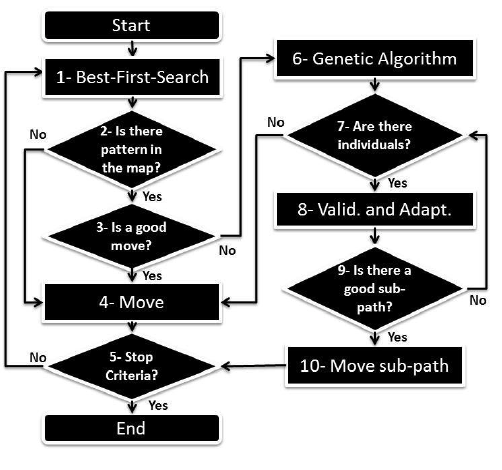
\includegraphics[keepaspectratio=true,scale=0.8]{ibagens/Fluxograma.png}
		\centering
		}
	\captionof{figure}{Fluxograma do PPGA \cite{Ulysses} }
	\label{fig:Fluxograma}
\end{minipage}
O modelo PPGA é dividido em 10 etapas:
\begin{enumerate}
	\item \textbf{Best-First-Seach} - Seleciona o nó atual e seleciona o menor valor na lista de nós abertos.
	\item \textbf{Existe um padrão?} - No modulo de AG existe uma contagem de proporção de vezes que sub-caminho são utilizados pelas tentativas de utilização, se essa proporção for baixa, é definido que não existe um padrão na busca, então, não utiliza o modulo de AG.
	\item \textbf{É um bom movimento?} - Verifica se o nó encontrado tem o valor menor que o atual, isto é, se aproxima mais do destino.
	\item \textbf{Movimento} - Adiciona o nó atual para a lista fechada.
	\item \textbf{Critério de parada?} - Se o ó atual é o nó de destino, o algoritmo termina, se não, continua para a próxima iteração.
	\item \textbf{Algoritmo genético} - É obtida apenas uma geração com os seguintes critérios:
	\begin{enumerate}
		\item A população inicial tem 4 indivíduos.
		\item Gera os primeiros descendentes utilizando com 4 primeiros indivíduos com um critério de 50\%.
		\item Gera os próximos descendentes utilizando, pela mutação da população inicial com um critério de 25\%.
		\item É calculado a aptidão para 12 indivíduos. O elemento utilizado na ultima geração recebe o valor valor.
	\end{enumerate}
	\item \textbf{Existem indivíduos?} - Verifica se existem indivíduos para serem avaliados na população. Se nenhum dos indivíduos forem validos, o algoritmo continua a manutenção do nó atual.
	\item \textbf{Validação e adaptação} - Ajuda a garantir ageração e adaptação de bons indivíduos.
	\item \textbf{Existe um bom sub-caminho?} - Os indivíduos gerados são testados, um em cada iteração, se não for um bom elemento, 'removido da lista da população.
	\item \textbf{Movimento para o sub-caminho} - O elemento será usado como um sub-caminho composto pelos nós que serão adicionados à lista fechada. O nó real se tornar o último nó do sub-caminho. Este elemento será inserido para a próxima geração do GA.
\end{enumerate}

A Figura \ref{fig:CaminhoPPGA} mostra o resultado de caminho percorrido pelo BFS (A) e o PPGA (B) em um mesmo ambiente simulado. 


\begin{minipage}{\linewidth}
	\makebox[\linewidth]{
		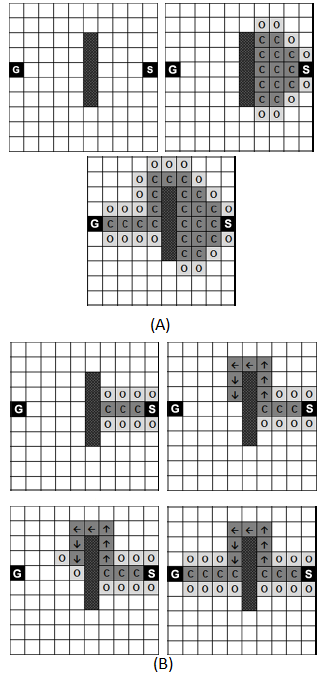
\includegraphics[keepaspectratio=true,scale=1.2]{ibagens/PPGA.png}
		\centering
		}
	\captionof{figure}{Caminho criado pelo BFS e o PPGA \cite{Ulysses} }
	\label{fig:CaminhoPPGA}
\end{minipage}

Os resultados obtidos da análise feita por \cite{Ulysses} do PPGA foram bons, por encontrar boas soluções em um curto período de tempo, mostrando ser muito bom para mapas onde o percurso segue um padrão, mas perdendo para o BFS para mapas mistos ou que não seguem o mesmo padrão ao longo o percurso, considerando o modelo como promissor, indicando que mudanças nos parâmetros do algoritmo genéticos, pode melhorar o desempenho dos testes \cite{Ulysses}.

\section{Algoritmos genéticos paralelos ou distribuídos para busca de caminhos}

Foi demonstrado que algoritmos genéticos paralelos são eficientes para a resolução de problemas de busca de caminho, tal como o clássico problema do caixeiro viajante, que consiste em dado um número finito de cidades com seus custos de viagem entre elas, deve-se encontrar o caminho mais curto para viajar entre todas as cidades e voltar ao ponto inicial. 

O problema pode ser representado pelo modelo de um grafo direcionado ponderado, aplicando a mesma ideia, o problema seria encontrar o caminho de menor custo para percorrer todos os nós, de maneira análoga, as cidades seriam os nós e a distancia entre elas, o peso das arestas \cite{Jason}\cite{Alaoui}\cite{Heinz}.

Os algoritmos genéticos exigem apenas o valor dado por uma função objetivo como parâmetro e mesmo sobre espaços de busca grandes, tem uma convergência rápida. Por causa do processo associado, agrega uma visão mais global do espaço de busca na prática de otimização e possuem uma fácil paralelização por causa da independência dos seus processos. Em comparação com as técnicas de busca mais comuns,que requerem informações derivadas, continuidade do espaço de busca ou conhecimento completo da função objetiva.\cite{Vilson}.

A solução para este tipo de problema pode requer uma quantidade grande de processamento. Uma boa solução seria dividir o processamento do problema em pequenas partes e distribuir cada parte para um processador a parte, trabalhando de forma distribuída ou paralela. Vários modelos para essa finalidade foram propostos.

Um modelo interessante para paralelização seria o de mestre-escravo, onde o mestre fica responsável na manutenção da população e execução dos operadores genéticos. A avaliação dos melhores indivíduos é distribuída para os demais escravos. O mestre envia um indivíduo a cada um dos escravos subjacentes. 

Cada escravo realiza a interpretação do problema, aplica a função de cálculo para a escolha dos melhores indivíduos e envia seus resultados ao mestre, que executa seleção dos indivíduos e a geração da nova população, repetindo o processo como um todo. Essa estrutura teve implicação satisfatória para a automação de design de circuitos eletrônicos\cite{Jason}. A Figura \ref{fig:AGParallelJohn} mostra o desenho do modelo proposto.

\begin{minipage}{\linewidth}
	\makebox[\linewidth]{
		\centering
		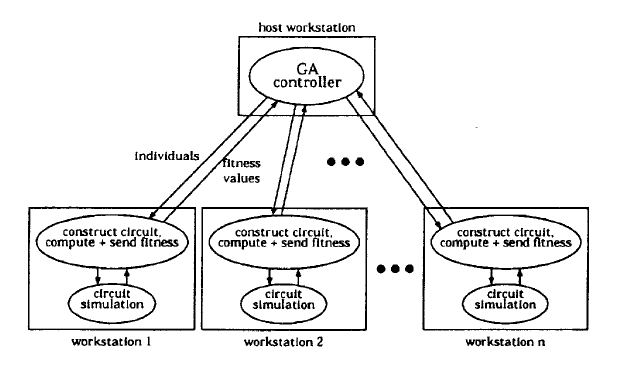
\includegraphics[keepaspectratio=true,scale=0.5]{ibagens/AGParallelJohn.png}
		\centering
		}
	\captionof{figure}{Desenho do modelo de \cite{Jason} }
	\label{fig:AGParallelJohn}
\end{minipage}

Outra forma de trabalhar com o modelo de mestre escravo, seria definir que cada um dos nós escravos subjacentes fica responsável por sua própria população. O nó central mestre, cria as populações iniciais e as distribui para os nós escravos. Cada nó escravo processa a evolução da população por um determinado número de gerações e então a submete ao mestre. O mestre então seleciona os melhores indivíduos dentre todas as populações dos nós escravos e os distribui novamente. 

Em cada nó escravo, os novos indivíduos distribuídos pelo mestre são inseridos na população corrente e o processo de evolução recomeça. A migração entre os escravos, que é controlado pelo nó mestre, implementa o mecanismo que regula a velocidade da convergência e oferece os meios de escape dos mínimos locais. Entretanto a migração das populações dos nós escravos para o mestre e vice versa pode impor um certo grau de sobre carga, dependente do meio de comunicação entre os nós. Esse modelo obteve sucesso no mapeamento de tarefas em maquinas paralelas. \cite{Alaoui}

Podemos partir do ponto que cada indivíduo é o responsável por encontrar e reproduzir com um parceiro em sua vizinhança. O controle de seleção e reprodução se espalha pela população e o algoritmo deixa de ser centralizado em um mestre, com isso, diminui o grau de sincronização e facilita a paralelização. 

O processo do algoritmo é definir uma representação genética para o problema e criar a estrutura de vizinhança e sua população inicial. Cada indivíduo faz uma busca em sua vizinhança e seleciona um parceiro para a reprodução. Uma geração descendente é criada com o operador genético resultante. \cite{Heinz}

Podemos observar alguns problemas nos modelos apresentados \cite{Vilson}, no modelo de \cite{Jason} existe problema em explorar o paralelismo no cálculo de verificação dos indivíduos não explorando para a reprodução e mutação. No modelo de \cite{Heinz}, tem a possibilidade de utilizar vários métodos de busca de indivíduos da mesma população, sendo úteis em casos que a eficiência dos métodos de busca se mostram dependentes da instancia do problema. 

O modelo \cite{Alaoui}, por todos os escravos devem enviar para o nó mestre, demanda uma grande capacidade de processamento no nó mestre, e proporciona a divisão das populações em pequenas ou de médio porte.

 \cite{Vilson} desenvolveu seu próprio modelo, utilizando o modelo de \cite{Alaoui} como inspiração. O modelo segue o conceito mestre-escravo, o mestre crias as populações e distribui a cada uma delas, os conjuntos de genes e parâmetros iniciais. O mestre é utilizado para a troca de indivíduos entre as populações, mantendo um indivíduo de cada população até serem substituídos por um melhor e envia esses indivíduos para as populações que não seja a sua de origem. 
 
 As populações são independentes, gerando seus indivíduos iniciais com base nos genes enviados pelo mestre, aplicando seus próprios operadores de evolução e a população que determina os parceiros dos indivíduos.
 A Figura \ref{fig:AGParallel} mostra o desenho do modelo.
 
 \begin{minipage}{\linewidth}
 	\makebox[\linewidth]{
 		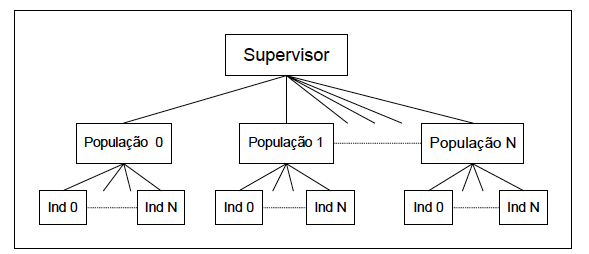
\includegraphics[keepaspectratio=true,scale=0.5]{ibagens/AGParallel.png}
 		\centering
 		}
 	\captionof{figure}{Protótipo de \cite{Vilson} }
 	\label{fig:AGParallel}
 \end{minipage}
 